%
% teil1.tex -- Beispiel-File für das Paper
%
% (c) 2020 Prof Dr Andreas Müller, Hochschule Rapperswil
%
% !TEX root = ../../buch.tex
% !TEX encoding = UTF-8
%
\section{Geostrophischer Wind
\label{geostrophisch:section:geoWind}}
\kopfrechts{Problemstellung}


\subsection{Coriolis-Kraft
\label{geostrophisch:subsection:coriolis}}
Die Coriolis-Kraft, welche durch die Rotation der Erde entsteht, beeinflusst die Bewegung von Luftmassen und anderen frei beweglichen Körpern auf der Erdoberfläche. Sie ist eine Scheinkraft, die nur in einem rotierenden Bezugssystem wie dem der Erde auftritt. Die Stärke hängt von der geografischen Breite ab und nimmt in Richtung der Pole zu.
Der Coriolis-Parameter $f$ beschreibt diese Abhängigkeit und ist definiert als 
\begin{equation}
f\, 
= 
2\Omega\sin(\phi)
\label{geostrophisch:equation1}.
\end{equation}
In dieser Gleichung steht $\Omega$ für die Winkelgeschwindigkeit der Erdrotation und $\phi$ für die geografische Breite auf der Erdoberfläche.
Die Coriolis-Kraft wirkt immer senkrecht zur Bewegungsrichtung. In der Meteorologie betrachtet man sie in der Regel pro Masseneinheit, da sich die Masse eines Luftpakets nicht eindeutig festlegen lässt. Auf der Nordhalbkugel lenkt sie Bewegungen nach rechts ab, auf der Südhalbkugel nach links. Mathematisch lässt sie sich für eine Geschwindigkeit $\vec{v}_g $ mit Hilfe des Kreuzproduktes darstellen. 
Die Coriolis-Kraft pro Masseneinheit ergibt sich aus der Formel
\begin{equation}
\frac{\vec{F}_c} {m}
= 
-f\, (\vec{k} \times \vec{v}_g) 
\label{geostrophisch:equation2},
\end{equation}
wobei $\vec{k}$ ein Einheitsvektor ist, der lokal in vertikaler Richtung, das heisst senkrecht zur Erdoberfläche (radial nach aussen vom Erdmittelpunkt), zeigt.
Das Kreuzprodukt von $\vec{k}$ mit  $\vec{v}_g $ sorgt dafür, dass die Coriolis-Kraft immer genau senkrecht zur Bewegungsrichtung wirkt.
%\begin{equation}
%\vec{k} =
%\left(
%\begin{array}{c}
%	0 \\
%	0 \\
%	1
%\end{array}
%\right)
%\label{geostrophisch:equation3}
%\end{equation}

\subsection{Gradientenkraft
\label{geostrophisch:subsection:gradient}}
Die Gradientenkraft ist die treibende Kraft pro Masseneinheit, die entsteht, wenn zwischen zwei Orten ein Druckunterschied besteht. Sie wirkt immer von Gebieten mit hohem Druck in Richtung niedrigen Drucks und ist die wichtigste antreibende Kraft für Luftbewegungen in der Atmosphäre. Je grösser der Druckunterschied über eine bestimmte Entfernung, desto stärker ist die Gradientenkraft.
Mathematisch lässt sie sich wie folgt beschreiben:
\begin{equation}
\frac{\vec{F}_p} {m}
= 
-\frac{1}{\rho} \nabla p
\label{geostrophisch:equation4},
\end{equation}
wobei $\rho$ die Luftdichte und $\nabla p$ der Druckgradient ist. 
Der negative Vorfaktor zeigt, dass die Kraft immer in Richtung des abnehmenden Drucks wirkt.

Die Gradientenkraft setzt Luftmassen in Bewegung, da sie ein Ungleichgewicht im Druckfeld ausgleicht. Ohne weitere Kräfte wie die Coriolis-Kraft würde die Luft somit direkt vom Hochdruckgebiet in das Tiefdruckgebiet strömen.
\subsection{Geostrophischer Wind}

Der geostrophische Wind ist eine idealisierte Luftströmung, bei der sich die Druckgradientkraft und die Coriolis-Kraft im Gleichgewicht befinden. In diesem Fall bewegt sich die Luft parallel zu den Isobaren (Linien gleichen Drucks). Auf der Nordhalbkugel befindet sich das Tiefdruckgebiet dabei stets zur linken Seite der Strömungsrichtung, auf der Südhalbkugel ist es umgekehrt.

Diese Näherung gilt besonders gut in der freien Atmosphäre oberhalb der Reibungsschicht (ca. 1 km Höhe), wo Reibungskräfte vernachlässigbar sind. 

\begin{figure}
    	\centering
    	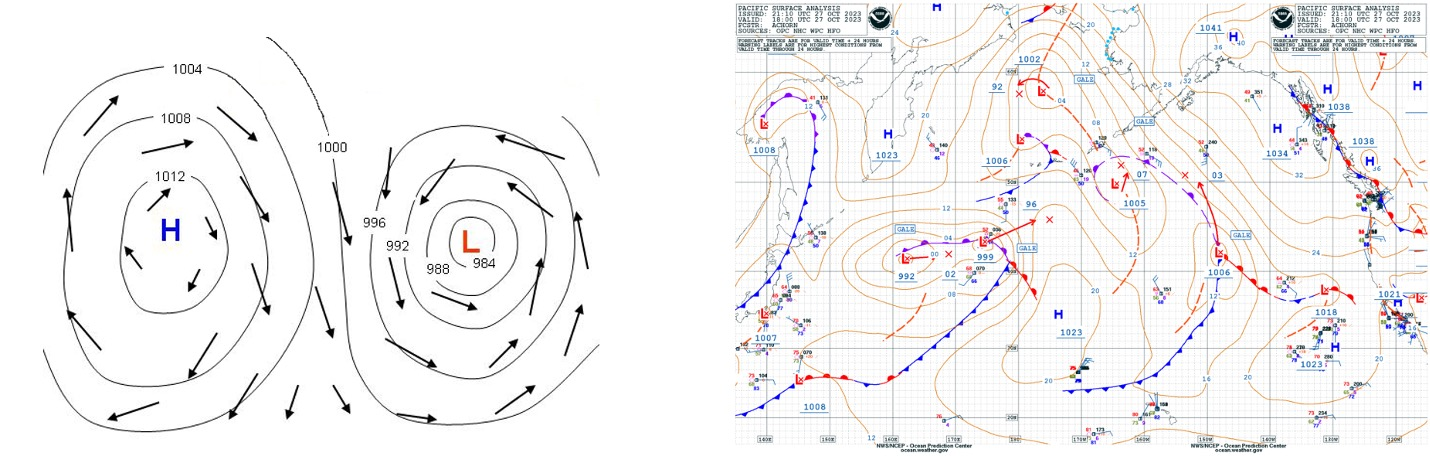
\includegraphics[scale=0.25]{geostrophisch_vs_real.jpg}
  	 \caption{Links: idealer geostrophischer Wind, parallel zu den Isobaren. Rechts: reale Wetterkarte mit Windpfeilen, die nicht exakt parallel zu den Isobaren verlaufen, zum Beispiel durch Reibung in Bodennähe.}
   	\label{bild:geostrophischvsreal}
\end{figure}

\begin{figure}
    	\centering
    	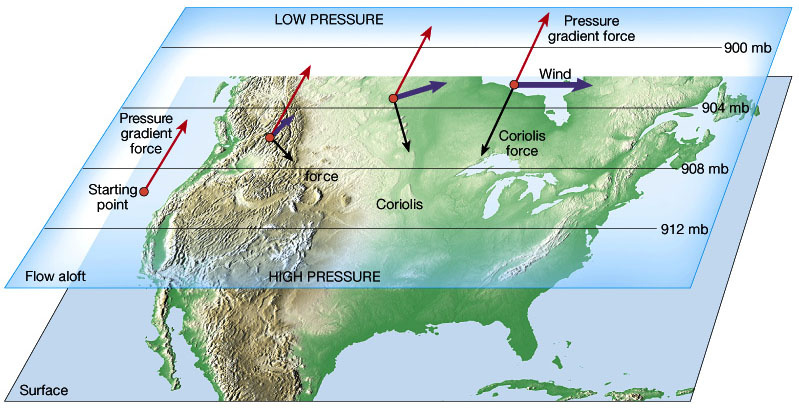
\includegraphics[scale=0.4]{Reibung.jpg}
  	 \caption{Eine grafische Darstellung, die den Einfluss von Reibung in Bodennähe zeigt. Die Einheit mb steht für Millibar. Heutzutage verwendet man hPa (Hektopascal). 1mb = 1hPa}
   	\label{bild:reibung}
\end{figure}


Wichtiger Hinweis zur Idealisierung:
Der geostrophische Wind ist ein nützliches Modell, um die grossskalige Strömung in der Atmosphäre zu beschreiben. In der Realität treten jedoch Abweichungen auf, insbesondere in Bodennähe, wo Reibung den Wind abbremst und in Richtung niedriger Drücke ablenkt. Auch komplexe Topografie und instationäre Wettersituationen können dazu führen, dass der Idealzustand nicht erreicht wird.
Diese Abweichungen werden in Abschnitt~\ref{geostrophisch:subsection:failedPrediction} (Grund der fehlerhaften Vorhersage) nochmals aufgegriffen.







